\documentclass{standalone}

\usepackage{ctex}
\usepackage{van-de-la-sehen}
\usepackage{tkz-euclide}
\usetikzlibrary{calc}
\usetkzobj{all}

\begin{document}

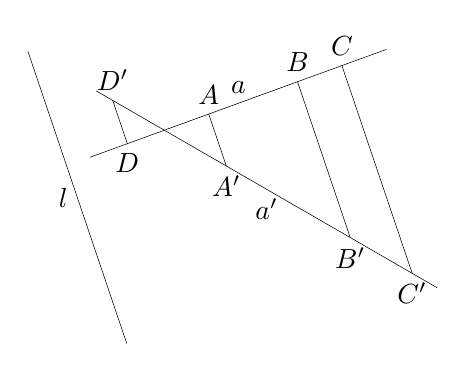
\begin{tikzpicture}[scale=0.5]

\tkzDefPoint(0,0){O}
\tkzDefPoint(150:4){P}
\tkzDefPoint(-100:5.5){Q}
\tkzDefPoint(150:2){U}
\tkzDefPoint(-30:8){V}
\tkzDefPoint(-160:2){X}
\tkzDefPoint(20:6){Y}
\tkzDefPointWith[linear,K=0.2](O,Y)\tkzGetPoint{A}
\tkzDefPointWith[linear,K=0.6](O,Y)\tkzGetPoint{B}
\tkzDefPointWith[linear,K=0.8](O,Y)\tkzGetPoint{C}
\tkzDefPointWith[linear,K=0.5](O,X)\tkzGetPoint{D}
\tkzDefLine[parallel=through A](P,Q)\tkzGetPoint{A''}
\tkzDefLine[parallel=through B](P,Q)\tkzGetPoint{B''}
\tkzDefLine[parallel=through C](P,Q)\tkzGetPoint{C''}
\tkzDefLine[parallel=through D](P,Q)\tkzGetPoint{D''}
\tkzInterLL(A,A'')(U,V) \tkzGetPoint{A'}
\tkzInterLL(B,B'')(U,V) \tkzGetPoint{B'}
\tkzInterLL(C,C'')(U,V) \tkzGetPoint{C'}
\tkzInterLL(D,D'')(U,V) \tkzGetPoint{D'}
\tkzDrawSegments(P,Q U,V X,Y A,A' B,B' C,C' D,D')
\tkzLabelLine[left](P,Q){$l$}
\tkzLabelLine[above](X,Y){$a$}
\tkzLabelLine[below](U,V){$a'$}
\tkzLabelPoints[above](D')
\tkzLabelPoints[below](D)
\tkzLabelPoints[below](A',B',C')
\tkzLabelPoints[above](A,B,C)

\end{tikzpicture}

\end{document}
